\documentclass{article}
\usepackage[utf8]{inputenc}
\usepackage[margin=1.0in]{geometry}
\usepackage{amsmath}
\usepackage{amssymb}
\usepackage{fancyhdr}
\usepackage{physics}
\usepackage{wrapfig}
\usepackage{hyperref}
\usepackage{multirow}
\usepackage{amsthm}
\usepackage{pgfplots}

\pgfplotsset{compat=1.16}



\renewcommand{\thesubsection}{\thesection\Alph{subsection}}
\renewcommand\qedsymbol{\square}



\title{Quantum Mechanics PS3}
\author{Joe Crowley}
\date{October 2020}

\pagestyle{fancy}
\renewcommand{\headrulewidth}{0pt}
\renewcommand{\footrulewidth}{1pt}

\fancyhf{}
\rhead{
Joe Crowley \\
Physics 215 \\
Problem Set 2\\
}
\rfoot{Page \thepage}

\begin{document}  

\section{SN 1.2}
\textit{Suppose a $2 \times 2$ matrix $X$ (not necessarily Hermitian or unitary) is written as
$$
X=a_{0}+\sigma \cdot \mathrm{a}
$$
where $a_{0}$ and $a_{1,2,3}$ are numbers.}
\subsection{}
\textit{How are $a_{0}$ and $a_{k}(k=1,2,3)$ related to $\mathbf{tr}(X)$ and $\mathbf{tr}\left(\sigma_{k} X\right) ?$}
\subsection{}
\textit{Obtain $a_{0}$ and $a_{k}$ in terms of the matrix elements $X_{i j}$}

\newpage

\section{SN 1.8}
\textit{Using the orthonormality of $|+\rangle$ and $|-\rangle,$ prove
$$
\left[S_{i}, S_{j}\right]=i \varepsilon_{i j k} \hbar S_{k}, \quad\left\{S_{i}, S_{j}\right\}=\left(\frac{\hbar^{2}}{2}\right) \delta_{i j}
$$
where
$$
\begin{array}{l}
S_{x}=\frac{\hbar}{2}(|+\rangle\langle-|+|-\rangle\langle+|), \quad S_{y}=\frac{i \hbar}{2}(-|+\rangle\langle-|+|-\rangle\langle+|) \\
S_{z}=\frac{\hbar}{2}(|+\rangle\langle+|-|-\rangle\langle-|)
\end{array}
$$}


\newpage

\section{SN 1.9}
\textit{Construct $|\mathbf{S} \cdot \hat{\mathbf{n}} ;+\rangle$ such that
$$
\mathbf{S} \cdot \hat{\mathbf{n}}|\mathbf{S} \cdot \hat{\mathbf{n}} ;+\rangle=\left(\frac{\hbar}{2}\right)|\mathbf{S} \cdot \hat{\mathbf{n}} ;+\rangle
$$
where $\hat{\mathbf{n}}$ is characterized by the angles shown in the accompanying figure. Express your answer as a linear combination of $|+\rangle$ and $|-\rangle .[$Note: The answer is
$$
\cos \left(\frac{\beta}{2}\right)|+\rangle+\sin \left(\frac{\beta}{2}\right) e^{i \alpha}|-\rangle
$$
But do not just verify that this answer satisfies the above eigenvalue equation. Rather, treat the problem as a straightforward eigenvalue problem. Also, do not use rotation operators, which we will introduce later in this book.$]$}


\newpage
\section{SN 1.10}
\textit{The Hamiltonian operator for a two-state system is given by
$$
H=a(|1\rangle\langle 1|-| 2\rangle\langle 2|+| 1\rangle\langle 2|+| 2\rangle\langle 1|)
$$
where $a$ is a number with the dimension of energy. Find the energy eigenvalues and the corresponding energy eigenkets $($as linear combinations of $|1\rangle and |2\rangle$ $)$.}

\newpage

\section{SN 1.11}
\textit{A two-state system is characterized by the Hamiltonian
$$
H=H_{11}|1\rangle\left\langle 1\left|+H_{22}\right| 2\right\rangle\langle 2|+H_{12}[|1\rangle\langle 2|+| 2\rangle\langle 1|]
$$
where $H_{11}, H_{22},$ and $H_{12}$ are real numbers with the dimension of energy, and |1\rangle and |2\rangle are eigenkets of some observable $(\neq H) .$ Find the energy eigenkets and the corresponding energy eigenvalues. Make sure that your answer makes good sense for $H_{12}=0 .$ (You need not solve this problem from scratch. The following fact may be used without proof:
$$
(\mathbf{S} \cdot \hat{\mathbf{n}})|\hat{\mathbf{n}} ;+\rangle=\frac{\hbar}{2}|\hat{\mathbf{n}} ;+\rangle
$$
with $|\hat{n} ;+\rangle$ given by
$$
|\hat{\mathbf{n}} ;+\rangle=\cos \frac{\beta}{2}|+\rangle+e^{i \alpha} \sin \frac{\beta}{2}|-\rangle
$$
where $\beta$ and $\alpha$ are the polar and azimuthal angles, respectively, that characterize $\hat{\mathbf{n}}$. }

\begin{figure}[h!]
    \centering
    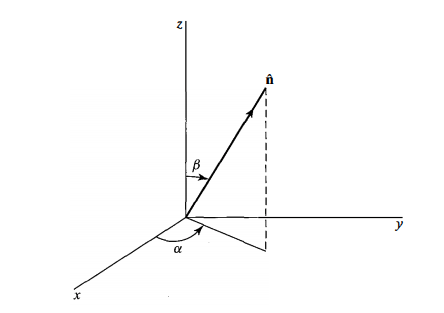
\includegraphics[width=0.4\textwidth]{figures/problem5.png}
    \label{fig:my_label}
\end{figure}

\newpage

\section{SN 1.12}
\textit{A spin $\frac{1}{2}$ system is known to be in an eigenstate of $\mathbf{S} \cdot \hat{\mathbf{n}}$ with eigenvalue $h / 2,$ where nis a unit vector lying in the $x z$ -plane that makes an angle $\gamma$ with the positive $z$ -axis.}
\subsection{}
\textit{Suppose $S_{x}$ is measured. What is the probability of getting $+\hbar / 2 ?$}

\subsection{}
\textit{Evaluate the dispersion in $S_{x}-$ that is,
$$
\left\langle\left(S_{x}-\left\langle S_{x}\right\rangle\right)^{2}\right\rangle
$$
(For your own peace of mind, check your answers for the special cases $\gamma=0$, $\pi / 2,$ and $\pi .)$}

\newpage


\section{SN 1.13}
\textit{A beam of $\operatorname{spin} \frac{1}{2}$ atoms goes through a series of Stern-Gerlach-type measurements as follows:}

\subsection{}
\textit{The first measurement accepts $s_{z}=h / 2$ atoms and rejects $s_{z}=-\hbar / 2$ atoms. }


\subsection{}
\textit{The second measurement accepts $s_{n}=h / 2$ atoms and rejects $s_{n}=-\hbar / 2$ atoms, where $s_{n}$ is the eigenvalue of the operator $\mathbf{S} \cdot \hat{\mathbf{n}},$ with $\hat{\mathbf{n}}$ making an angle $\beta$ in the $x z$ -plane with respect to the $z$ -axis.}


\subsection{}
\textit{The third measurement accepts $s_{z}=-\hbar / 2$ atoms and rejects $s_{z}=\hbar / 2$ atoms.}

\subsection*{}
\textit{What is the intensity of the final $s_{z}=-\hbar / 2$ beam when the $s_{z}=\hbar / 2$ beam surviving the first measurement is normalized to unity? How must we orient the second measuring apparatus if we are to maximize the intensity of the final $s_{z}=-\hbar / 2$ beam?}


\newpage

\section{SN 1.19}


\subsection{}
\textit{Compute
$$
\left\langle\left(\Delta S_{x}\right)^{2}\right\rangle \equiv\left\langle S_{2}^{x}\right\rangle-\left\langle S_{x}\right\rangle^{2}
$$
where the expectation value is taken for the $S_{z}+$ state. Using your result, check the generalized uncertainty relation
$$
\left\langle(\Delta A)^{2}\right\rangle\left\langle(\Delta B)^{2}\right\rangle \geq \frac{1}{4}|\langle[A, B]\rangle|^{2}
$$
with $A \rightarrow S_{x}, B \rightarrow S_{y}$}


\subsection{}
\textit{Check the uncertainty relation with $A \rightarrow S_{x}, B \rightarrow S_{y}$ for the $S_{x}+$ state.}

\newpage
\section{SN 1.20}
\textit{Find the linear combination of $|+\rangle$ and $|-\rangle$ kets that maximizes the uncertainty product
$$
\left\langle\left(\Delta S_{x}\right)^{2}\right\rangle\left\langle\left(\Delta S_{y}\right)^{2}\right\rangle
$$
Verify explicitly that for the linear combination you found, the uncertainty relation for $S_{x}$ and $S_{y}$ is not violated.}


\newpage

\section{SN 1.23}
\textit{Consider a three-dimensional ket space. If a certain set of orthonormal kets-say, $|1\rangle,|2\rangle,$ and $|3\rangle-$ are used as the base kets, the operators $A$ and $B$ are represented by
$$
A \doteq\left(\begin{array}{ccc}
a & 0 & 0 \\
0 & -a & 0 \\
0 & 0 & -a
\end{array}\right), \quad B \doteq\left(\begin{array}{ccc}
b & 0 & 0 \\
0 & 0 & -i b \\
0 & i b & 0
\end{array}\right)
$$ with $a$ and $b$ both real.}

\subsection{}
\textit{Obviously $A$ exhibits a degenerate spectrum. Does $B$ also exhibit a degenerate spectrum?}

Show that $A$ and $B$ commute.

Find a new set of orthonormal kets that are simultaneous eigenkets of both $A$ and $B .$ Specify the eigenvalues of $A$ and $B$ for each of the three eigenkets. Does your specification of eigenvalues completely characterize each eigenket?


\newpage
\section{SN 1.26}
\textit{Construct the transformation matrix that connects the $S_{z}$ diagonal basis to the $S_{x}$ diagonal basis. Show that your result is consistent with the general relation
$$
U=\sum_{r}\left|b^{(r)}\right\rangle\left\langle a^{(r)}\right|
$$}
\end{document}
